\chapter{Indústria brasileira de Jogos Eletrônicos}

A indústria de jogos no Brasil tem se consolidado como um dos maiores mercados consumidores do mundo, ocupando atualmente a quinta posição global em consumo de jogos eletrônicos. Dados recentes apontam que 89,8\% da população brasileira consome jogos regularmente (\cite{internetGame:share}), utilizando dispositivos móveis, consoles e computadores como principais plataformas. Essa alta adesão reflete a popularidade dos jogos eletrônicos no país, que ultrapassaram a barreira do entretenimento e se tornaram parte do cotidiano de grande parte dos brasileiros.

Entretanto, apesar da expressiva participação no consumo, o Brasil enfrenta desafios significativos quando se trata de publicação de jogos. Publicadoras de jogos, responsáveis por financiar, distribuir e promover os títulos no mercado, desempenham um papel crucial no sucesso de um jogo. Essas empresas frequentemente definem o alcance e o impacto que um título pode ter globalmente. Contudo, o Brasil não figura nem entre os dez principais países que mais publicam jogos (\cite{publishers:country}), evidenciando uma discrepância significativa entre o consumo e a produção nacional.

\begin{figure}[H]
    \centering
    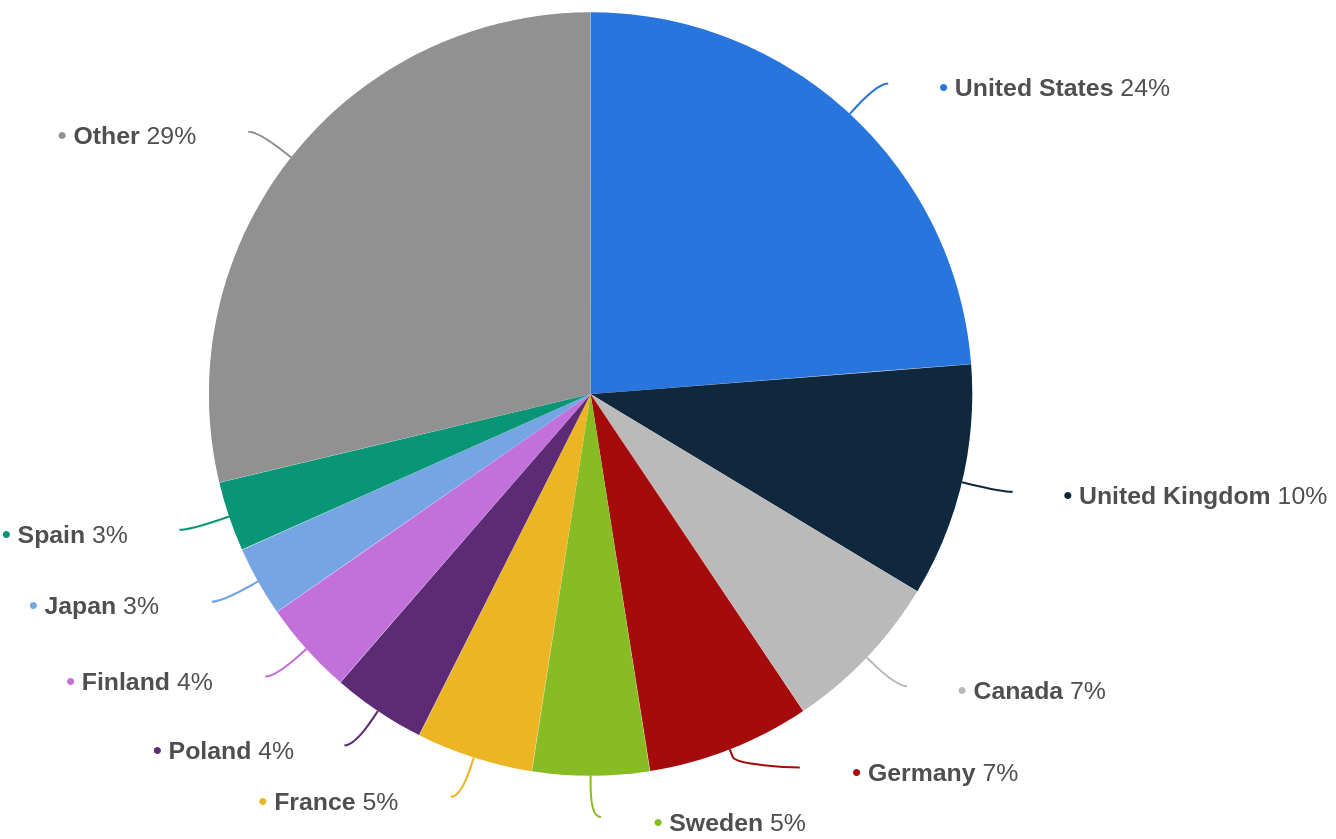
\includegraphics[width=0.8\textwidth]{figuras/Devs by Country.png}
    \caption{Distribuição de publicadoras de jogos por país. Fonte: \cite{publishers:country}}
    \label{fig:jogos-brasil}
\end{figure}

\section{História e evolução}
Historicamente, a indústria brasileira de jogos foca em títulos independentes e projetos de menor escala, devido às limitações de financiamento e infraestrutura. Embora existam exemplos notáveis de jogos brasileiros que alcançaram sucesso internacional, como \textit{Horizon Chase Turbo}\label{Língua estrangeira} e \textit{Chroma Squad}, os gêneros mais explorados tendem a ser aventura, RPG e simuladores, enquanto outros segmentos, como o de jogos de corrida no estilo \textit{Mario Kart} (com elementos de trapaça e apelo competitivo), ainda são pouco explorados.

Esse cenário oferece tanto desafios quanto, oportunidades para desenvolvedores brasileiros. De um lado, a falta de grandes publicadoras locais dificulta o alcance global dos títulos nacionais. Por outro lado, o imenso potencial criativo e a crescente comunidade de desenvolvedores no Brasil sugerem que o mercado pode se expandir significativamente, caso receba os investimentos e apoios necessários. Além disso, a criação de jogos que dialoguem com a identidade cultural brasileira pode ser um diferencial estratégico, atraindo tanto o público nacional quanto internacional.

Ao propor o desenvolvimento do \textit{USP Kart}, este trabalho busca não apenas explorar as possibilidades técnicas e criativas do desenvolvimento de jogos, mas também contribuir para a diversificação do mercado nacional. O objetivo é oferecer uma experiência de jogo de alta qualidade que valorize elementos culturais e acadêmicos brasileiros, demonstrando que o país possui capacidade técnica e artística para competir em segmentos atualmente pouco explorados.

\section{Títulos nacionais}
Apesar dos desafios enfrentados pela indústria brasileira de jogos, diversos títulos nacionais têm se destacado nos últimos anos, tanto no mercado interno quanto no internacional. Jogos como \textit{Horizon Chase Turbo}, \textit{Chroma Squad}, \textit{Dandara} e \textit{Aritana e a Pena da Harpia} são exemplos de produções brasileiras que conquistaram reconhecimento global, recebendo prêmios e críticas positivas da imprensa especializada.

Esses títulos demonstram a diversidade e a qualidade dos jogos produzidos no Brasil, abordando temas variados e explorando mecânicas inovadoras. Além disso, esses jogos frequentemente refletem a cultura e a identidade brasileira, apresentando elementos visuais e narrativos que dialogam com o público nacional e internacional. Um exemplo notável é o "Horizon Chase Turbo - Senna Forever", que homenageia o piloto brasileiro Ayrton Senna e destaca elementos culturais brasileiros.

\begin{figure}[H]
    \centering
    
\includegraphics[width=0.8\textwidth]{figuras/Horizon Chase Turbo - Senna.jpg}
    \caption{Homenagem ao piloto brasileiro, Ayrton Senna no jogo Horizon Chase Turbo. \cite{horizonChaseTurbo}}
    \label{fig:horizon-chase-turbo-senna}
\end{figure}

\subsection{Horizon Chase Turbo}
\textit{Horizon Chase Turbo} é um jogo de corrida desenvolvido pela Aquiris Game Studio, lançado em 2018 para múltiplas plataformas. Inspirado em clássicos dos anos 80 e 90, como \textit{Out Run} e \textit{Top Gear}, o jogo combina gráficos 3D modernos com jogabilidade arcade, oferecendo uma experiência nostálgica e desafiadora para os jogadores.

Como o \textit{USP Kart}, \textit{Horizon Chase Turbo} é um jogo de corrida que busca recriar a diversão e a emoção dos jogos clássicos do gênero. A estética retrô e a jogabilidade acessível são elementos-chave do jogo, que conquistou tanto fãs de longa data quanto novos jogadores.

Apesar das semelhanças, \textit{Horizon Chase Turbo} e \textit{USP Kart} diferem em suas abordagens como um jogo de corrida, sendo o gênero de corridas em Kart um subgênero de jogos de corrida que se destaca por sua jogabilidade acessível e dinâmica. Enquanto \textit{Horizon Chase Turbo} foca em corridas de carros clássicos em pistas realistas, \textit{USP Kart} explora mecânicas de combate e interação entre jogadores, inspiradas em títulos como \textit{Mario Kart}.

\begin{figure}[H]
    \centering
    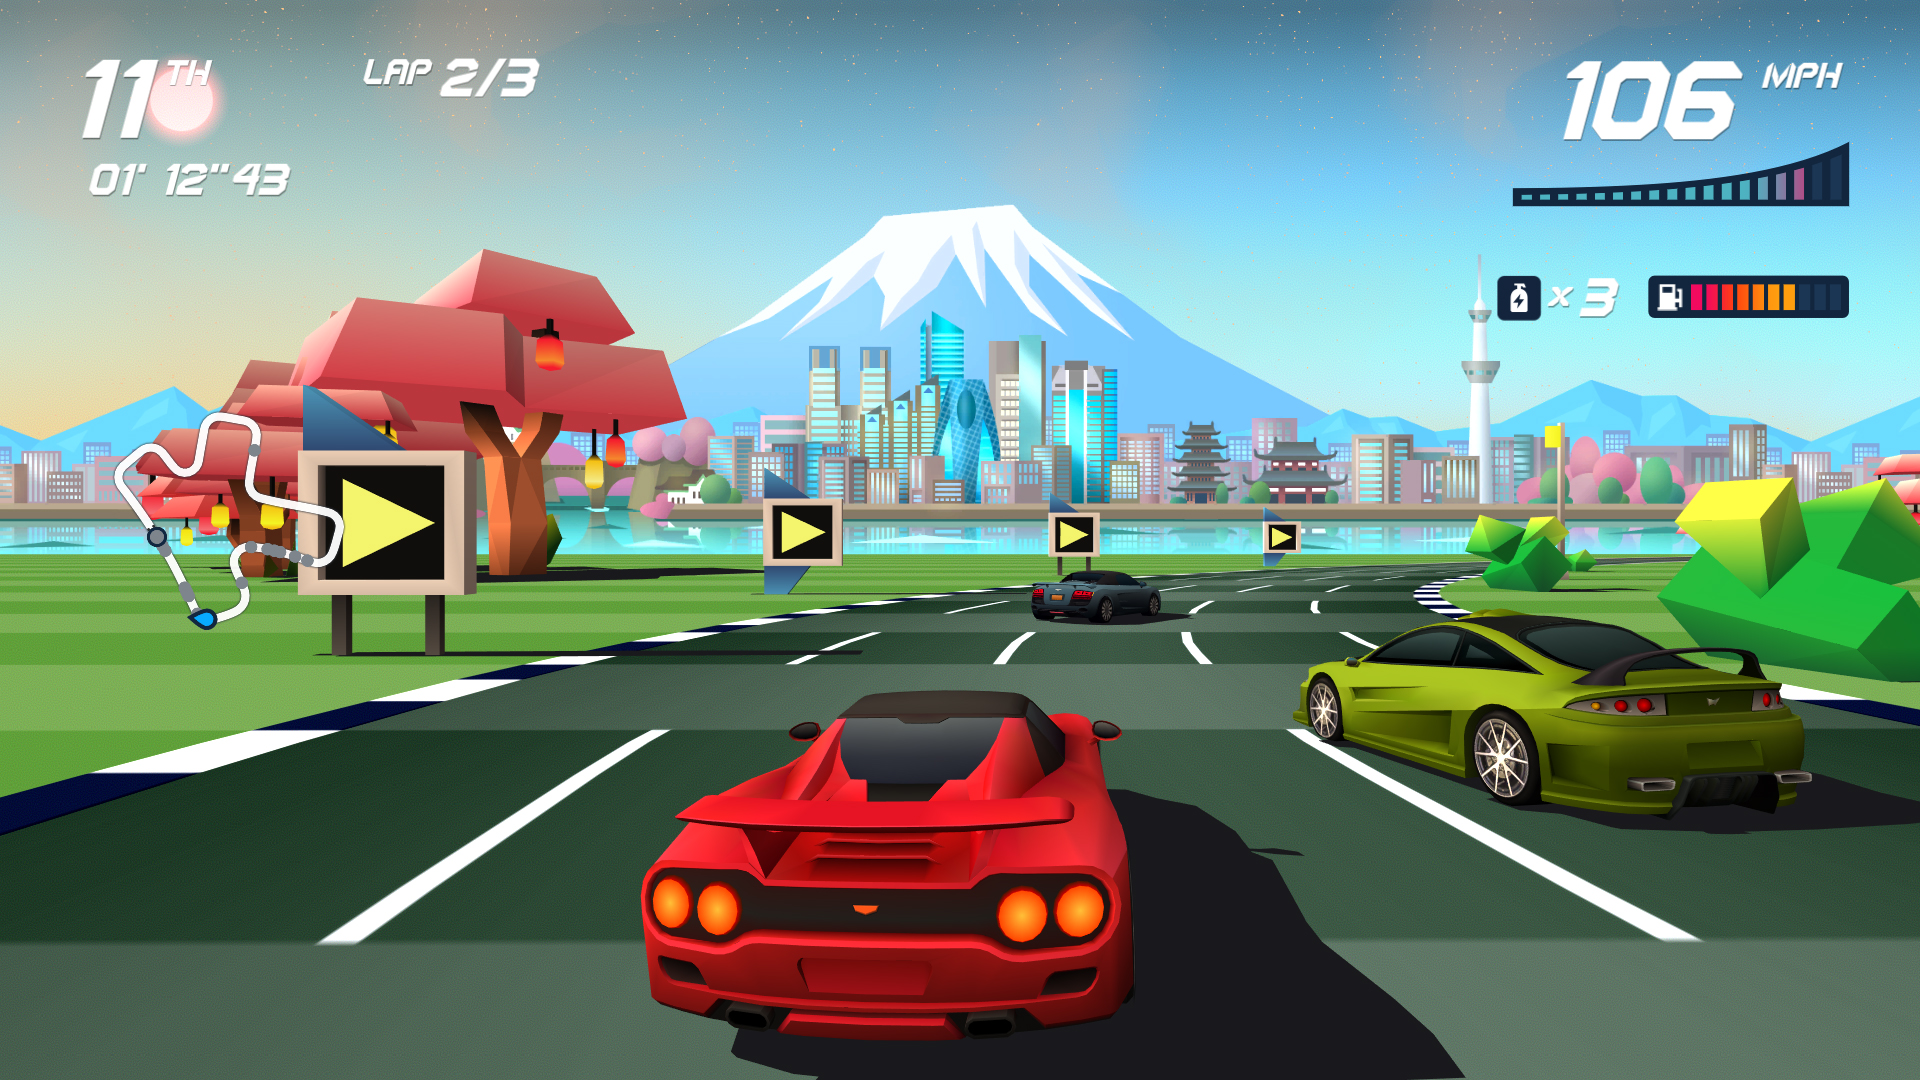
\includegraphics[width=0.8\textwidth]{figuras/Horizon Chase Turbo.jpeg}
    \caption{Horizon Chase Turbo. Fonte: \cite{horizonChaseTurbo}}
    \label{fig:horizon-chase-turbo}
\end{figure}

\subsection{Chroma Squad}
\textit{Chroma Squad} é um jogo de estratégia desenvolvido pela Behold Studios, lançado em 2015 para múltiplas plataformas. O jogo coloca o jogador no papel de um produtor de um programa de TV sobre super-heróis, permitindo que ele controle os personagens, cenários e enredos das batalhas.

\textit{Chroma Squad} é um exemplo de jogo brasileiro que se destaca pela criatividade e originalidade de sua proposta. A mistura de elementos de estratégia, simulação e RPG, combinada com uma narrativa envolvente e humorística, conquistou tanto a crítica quanto o público, tornando-se um dos títulos mais populares da Behold Studios.

\begin{figure}[H]
    \centering
    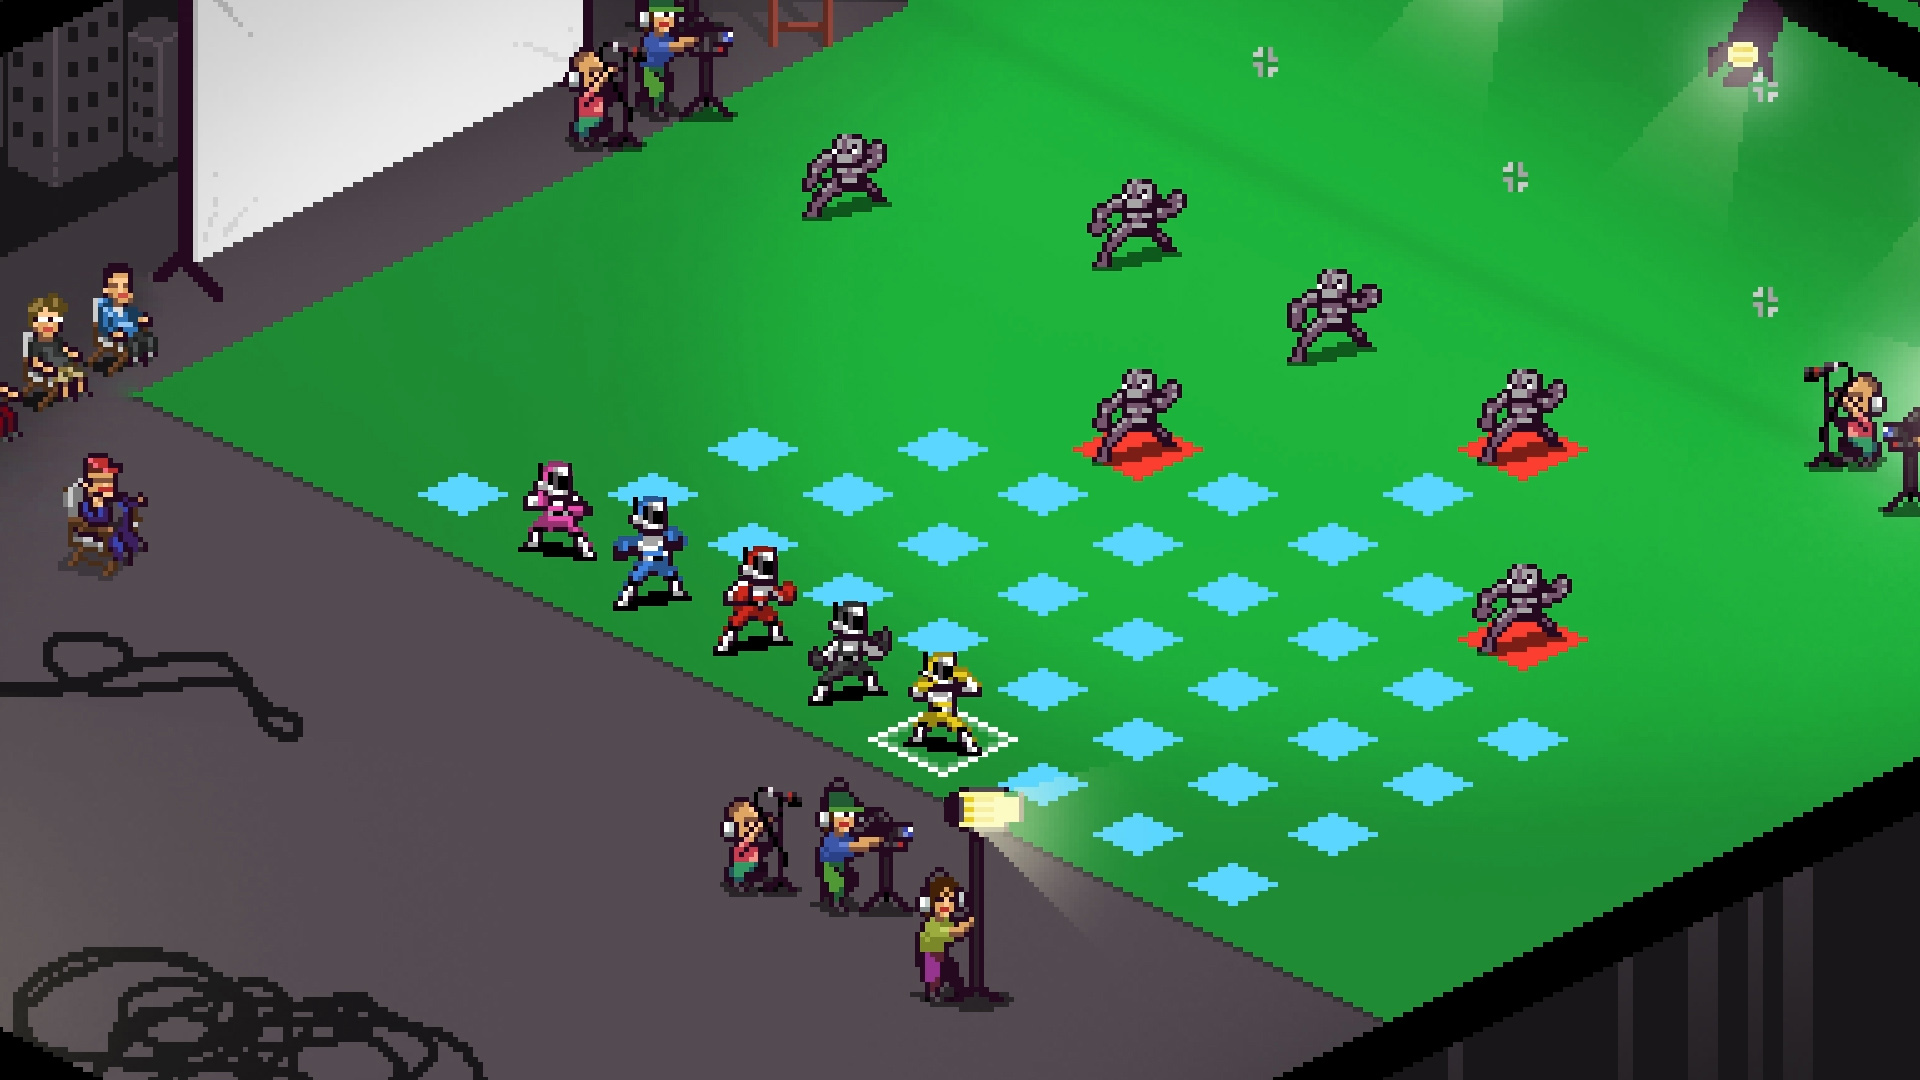
\includegraphics[width=0.8\textwidth]{figuras/Chroma Squad.jpg}
    \caption{Chroma Squad. Fonte: \cite{chromaSquad}}
    \label{fig:chroma-squad}
\end{figure}

\subsection{Dandara}
\textit{Dandara} é um jogo de ação e aventura desenvolvido pela Long Hat House, lançado em 2018 para múltiplas plataformas. O jogo apresenta uma jogabilidade única, baseada em movimentos de plataforma e combate, combinada com uma narrativa inspirada na cultura e história brasileira.

\textit{Dandara} é um exemplo de jogo brasileiro que se destaca pela qualidade de sua produção e pela originalidade de sua proposta. A estética visual e sonora do jogo, inspirada na cultura afro-brasileira, e a jogabilidade inovadora, que desafia os padrões do gênero, conquistaram a crítica e o público, tornando-se um dos títulos mais aclamados da Long Hat House.

\begin{figure}[H]
    \centering
    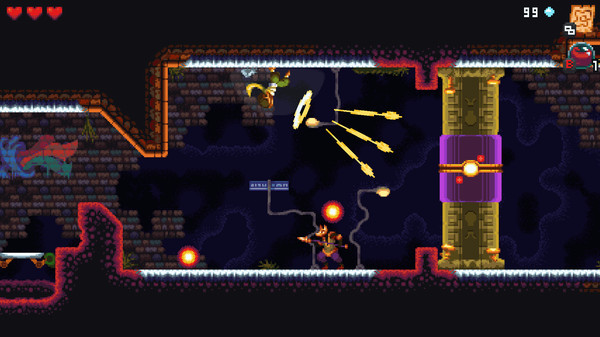
\includegraphics[width=0.8\textwidth]{figuras/Dandara.jpg}
    \caption{Dandara. Fonte: \cite{dandara}}
    \label{fig:dandara}
\end{figure}

\subsection{Aritana e a Pena da Harpia}
\textit{Aritana e a Pena da Harpia} é um jogo de ação e aventura desenvolvido pela Duaik Entertainment, lançado em 2014 para múltiplas plataformas. O jogo apresenta uma narrativa inspirada na mitologia indígena brasileira, combinada com uma jogabilidade baseada em movimentos de plataforma e combate.

\textit{Aritana e a Pena da Harpia} é um exemplo de jogo brasileiro que se destaca pela originalidade de sua proposta e pela qualidade de sua produção. A estética visual e sonora do jogo, inspirada na cultura indígena brasileira, e a narrativa envolvente, que explora temas como amizade, coragem e respeito à natureza, conquistaram a crítica e o público, tornando-se um dos títulos mais populares da Duaik Entertainment.

\begin{figure}[H]
    \centering
    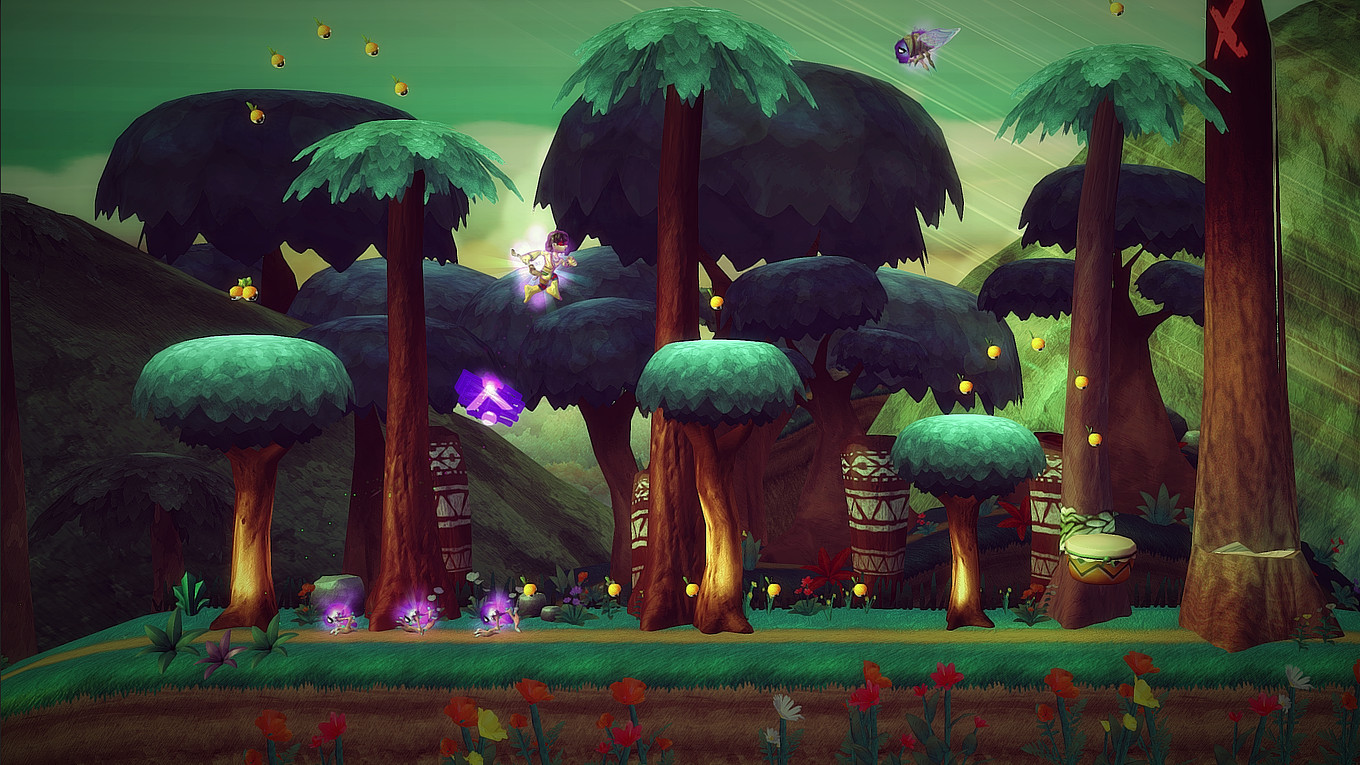
\includegraphics[width=0.8\textwidth]{figuras/Aritana.jpg}
    \caption{Aritana e a Pena da Harpia. Fonte: \cite{aritana}}
    \label{fig:aritana}
\end{figure}